\chapter{Introduzione}
\label{cap:introduzione}

In questo capito viene introdotto il problema per il quale è stato affrontato questo percorso di stage.
Viene descritto brevemente come è stato risolto seguendo i diversi vincoli imposti dall'azienda presso la quale ho sviluppato il progetto.
Viene presentata l'azienda presso la quale e viene descritta la struttura del documento.

\section{Analisi del problema}
C'è sempre più bisogno di ottenere informazioni da grandi quantità di documenti in una maniera rapida e semplice.
Il progetto sviluppato in questo percorso di stage è stato incentrato proprio su questa problematica: andando avanti nel tempo si accumulano moltissimi documenti e dover cercare una singola informazione all'interno delle volte può risultare scomodo.
Uno degli approcci più diretti per una persona per cercare un informazione qualsiasi, nella quotidianità, è quella di porre domande ad altre persone.
L'azienda presso quale ho svolto lo stage, per far sì che questo problema possa essere risolto tramite quest'ultimo approccio, ha deciso di sfruttare la potenza dei RALM. \\

\subsection{RALM}
I \gls{LLM} sono dei modelli di apprendimento automatico in grado di generare testi coerenti e informativi.
Hanno rivoluzionato il campo dei \gls{NLP} e vengono impiegati in diverse applicazioni, un esempio possono essere i chatbot.
Questi ultimi sfruttano la capacità dei LLM di interagire tramite il linguaggio naturale con gli utenti.
I Retrieval Augmented Language Model (RALM) non sono altro che dei LLM, basati sul \emph{\gls{question answering}}\glsfirstoccur, che permettono di utilizzare una fonte esterna di conoscenza (come ad esempio una collezione di documenti)
per fornire informazioni aggiuntive al modello durante la generazione di testo.
\noindent Un documento viene suddiviso in parti più piccole chiamate chunk. 
Il modello effettua una query alla fonte esterna usando l'input dell'utente come chiave di ricerca e riceve una lista formata da un numero determinato di chunk rilevanti (possono avere la risposta al quesito posto).
Il numero determinato di chunk viene dato dalla quantità di \emph{\gls{token}}\glsfirstoccur (elemento individuale all'interno di un testo: parola, parte di parola, punteggiatura) che il modello può ricevere in ingersso.
Questi chunk vengono poi utilizzati come contesto aggiuntivo e vengono combinati con l'input originale per produrre il testo finale.
Questo approccio permette di generare testi più informativi, accurati e diversificati sfruttando la conoscenza dovuta alla presenza della fonte esterna.

\subsection{Il problema}
Per poter garantire la qualità delle risposte generate dal RALM è necessario che i documenti a disposizione siano in formato testuale e che il loro contenuto abbia tutta l'informazione 
neccessaria.
I documenti sono disponibili in diversi formati e spesso non sono costituiti semplicemente di testo non strutturato, ma presentano frequentemente vari
"elementi semantici" come tabelle, immagini e titoli.
Presentano quindi informazione che non era immediatamente estraibile e convertibile in testo (tramite i tool di estrazione del contenuto) utile ai fini dell'interazione col RALM. \\
Un altro problema che si può presentare è che i chunk rilevanti forniti al RALM non sempre contengono la risposta alla domanda posta, quindi, effettivamente, non sempre sono veramente rilevanti.
L'ultimo problema affrontato è che spesso i documenti presentano elementi ripetuti come, ad esempio, una serie di punti presente in un indice (come mostrato in figura \ref{fig:reps}).
Queste ripetizioni occuperebbero spazio inutilmente all'interno dei chunk aumentando così il numero di questi ultimi.

\begin{figure}[!h]
    \centering
    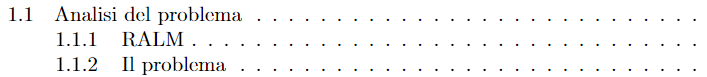
\includegraphics[width=0.8\columnwidth]{images/esempioIndice.png}
    \caption{Esempio di elementi ripetuti da minimizzare nella conversione del contenuto.}
    \label{fig:reps}
\end{figure}

\subsection{Il progetto}
Gli elementi sui quali mi sono concentrato di più per migliorare la qualità delle risposte fornite dal RALM sono state le tabelle e i titoli.
Ho applicato un metodo di conversione delle tabelle in modo tale da poterle rendere comprensibili al RALM e che potessero comunque mantenere il senso della loro struttura anche se sottoforma di testo non strutturato. \\
Per migliorare la probabilità di trovare chunk rilevanti vengono aggiunti i titoli ai chunk (ove possibile) in modo tale da potergli dare un senso di posizione all'interno del documento. \\
Le ripetizioni di caratteri vengono semplicemente ridotte a un singolo carattere.

\section{L'azienda: Siav S.p.A.}

\begin{figure}[!h] 
    \centering 
    
\includegraphics[width=0.5\columnwidth]{images/logoSiav.jpg} 
    \caption{Logo dell'azienda Siav S.p.A.}
\end{figure}
Siav S.p.A. è un’azienda informatica specializzata nella dematerializzazione, nella gestione elettronica dei documenti e nei processi digitali.
Fondata nel 1990 a Rubano (Padova) è oggi la prima azienda italiana nel settore dell’Enterprise Content Management, e offre software, soluzioni in cloud e servizi di outsourcing per la Gestione Elettronica dei Documenti, il Protocollo Informatico, il Workflow Management, la Fatturazione Elettronica e la Conservazione Digitale.



\section{Organizzazione del testo}

\begin{description}
    \item[{\hyperref[cap:analisi-preliminare]{Il secondo capitolo}}] decrive gli obiettivi nel dettaglio e mostra le varie soluzioni applicate per poter rendere migliore la qualità delle risposte del RALM;
    
    \item[{\hyperref[cap:progettazione-codifica]{Il terzo capitolo}}] approfondisce le tecnologie utilizzate nel progetto, la progettazione e la codifica di quanto sviluppato;
    
    \item[{\hyperref[cap:verifica-validazione]{Il quarto capitolo}}] illustra i vari test effettuati sul RALM e mostra i risultati ottenuti ogni modifica attuata;
    
    \item[{\hyperref[cap:conclusioni]{Nel quinto capitolo}}] vengono scritte le conclusioni riguardo al progetto svolto.
\end{description}

Riguardo la stesura del testo, relativamente al documento sono state adottate le seguenti convenzioni tipografiche:
\begin{itemize}
	\item gli acronimi, le abbreviazioni e i termini ambigui o di uso non comune menzionati vengono definiti nel glossario, situato alla fine del presente documento; 
	\item per la prima occorrenza dei termini riportati nel glossario viene utilizzata la seguente nomenclatura: \emph{parola}\glsfirstoccur;
\end{itemize}
